\documentclass[border=10pt]{standalone}
\usepackage[svgnames]{xcolor}
\usepackage{amsmath}
\usepackage{pgfplots}
\pgfplotsset{compat=newest}
\usepackage[sfdefault]{FiraSans}
\usepackage{FiraMono}
\renewcommand*\familydefault{\sfdefault}
\begin{document}
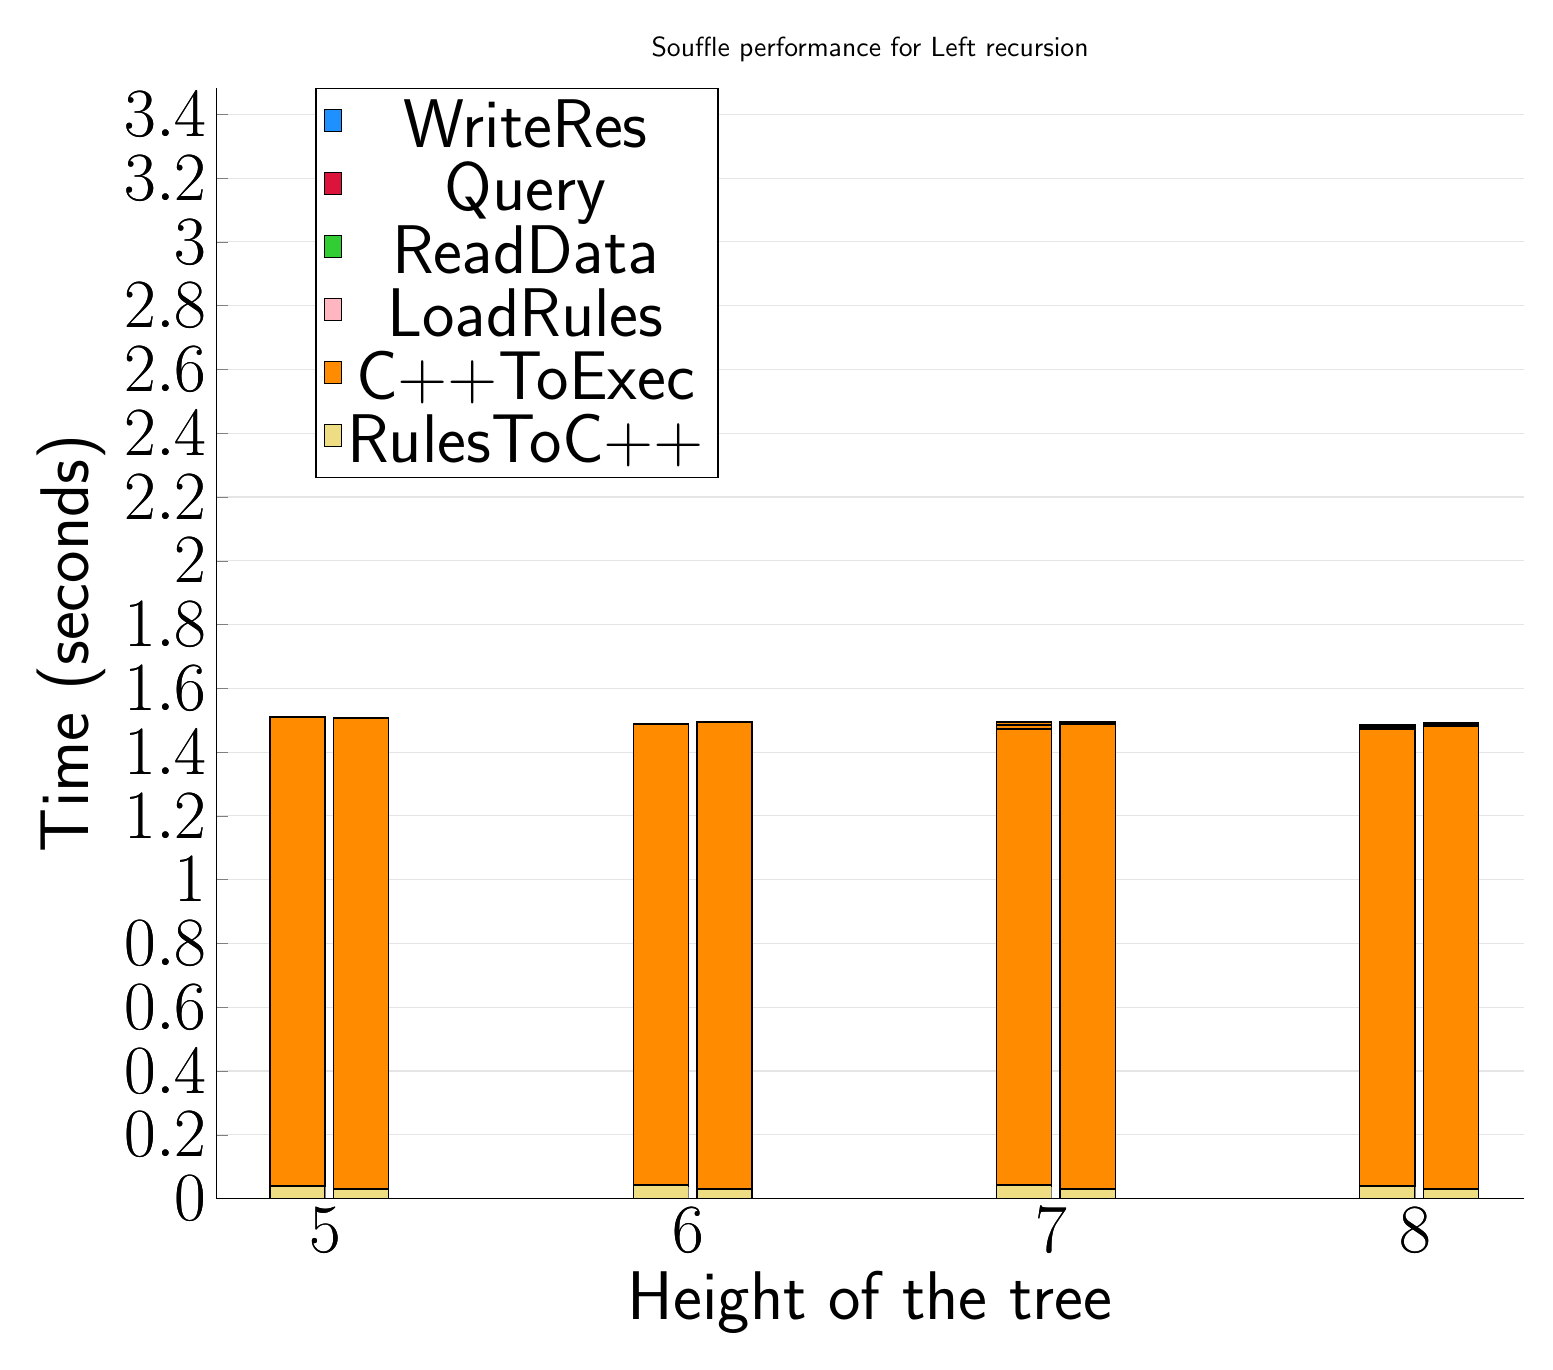
\begin{tikzpicture}
\begin{axis}[
   ybar stacked,
   title={Souffle performance for Left recursion},
   bar shift=-10pt,
   width=1.5\textwidth,
   bar width=0.7cm,
   ymajorgrids, tick align=inside,
   major grid style={draw=gray!20},
   xtick=data,
   ymin=0, ymax=3.4829999685287474,
   axis x line*=bottom,
   axis y line*=left,
   enlarge x limits=0.1,
   legend style={
       at={(0.23, 1)},
       anchor=north,
       legend columns=1,
       font=\Huge,
   },
   ylabel={Time (seconds)},
   xlabel={Height of the tree},
   label style={font=\Huge},
   tick label style={font=\Huge},
]
\addlegendimage{fill=DodgerBlue, draw=black, line width=0.2pt}
\addlegendentry{WriteRes}
\addlegendimage{fill=Crimson, draw=black, line width=0.2pt}
\addlegendentry{Query}
\addlegendimage{fill=LimeGreen, draw=black, line width=0.2pt}
\addlegendentry{ReadData}
\addlegendimage{fill=LightPink, draw=black, line width=0.2pt}
\addlegendentry{LoadRules}
\addlegendimage{fill=DarkOrange, draw=black, line width=0.2pt}
\addlegendentry{C++ToExec}
\addlegendimage{fill=LightGoldenrod, draw=black, line width=0.2pt}
\addlegendentry{RulesToC++}
\addplot +[fill=LightGoldenrod, draw=black, line width=0.5pt] coordinates {
    (5, 0.039999985694885255)
    (6, 0.04200000762939453)
    (7, 0.040999984741210936)
    (7, 0.04100005626678467)
    (7, 0.043999981880187986)
    (8, 0.039999985694885255)
    (8, 0.04100000858306885)
    (8, 0.040000081062316895)
};
\addplot +[fill=DarkOrange, draw=black, line width=0.5pt] coordinates {
    (5, 1.4690000057220458)
    (6, 1.4450000286102296)
    (7, 1.444000005722046)
    (7, 1.431999969482422)
    (7, 1.4490000247955321)
    (8, 1.4410000324249268)
    (8, 1.4379999876022338)
    (8, 1.4319999456405639)
};
\addplot +[fill=LightPink, draw=black, line width=0.5pt] coordinates {
    (5, 0.00012445430000000002)
    (6, 0.0001129541)
    (7, 0.00012539989999999998)
    (7, 0.0001254333)
    (7, 0.000123675)
    (8, 0.0001253666)
    (8, 0.000123954)
    (8, 0.00012332489999999997)
};
\addplot +[fill=LimeGreen, draw=black, line width=0.5pt] coordinates {
    (5, 0.0003095541)
    (6, 0.00038438740000000006)
    (7, 0.0005189667000000001)
    (7, 0.0005282084)
    (7, 0.0005262248)
    (8, 0.0008084127999999999)
    (8, 0.0007981289)
    (8, 0.0008098207999999999)
};
\addplot +[fill=Crimson, draw=black, line width=0.5pt] coordinates {
    (5, 0.0001454459)
    (6, 0.0003247876)
    (7, 0.0007475375999999999)
    (7, 0.0007871957000000001)
    (7, 0.0007793915999999999)
    (8, 0.001892764)
    (8, 0.0018636159999999998)
    (8, 0.0018687119999999998)
};
\addplot +[fill=DodgerBlue, draw=black, line width=0.5pt] coordinates {
    (5, 0.00027744989999999996)
    (6, 0.0005345294000000001)
    (7, 0.0006392539999999999)
    (7, 0.0005194791)
    (7, 0.0005409416000000001)
    (8, 0.0012149918)
    (8, 0.0009246667999999999)
    (8, 0.0010122002)
};
\end{axis}
\begin{axis}[
   ybar stacked,
   bar shift=13pt,
   width=1.5\textwidth,
   bar width=0.7cm,
   ymajorgrids, tick align=inside,
   major grid style={draw=none},
   xtick=data,
   ymin=0, ymax=3.4829999685287474,
   axis x line*=none,
   axis y line*=none,
   enlarge x limits=0.1,
   label style={font=\Huge},
   tick label style={font=\Huge},
]
\addplot +[fill=LightGoldenrod, draw=black, line width=0.5pt] coordinates {
    (5, 0.030000000000000006)
    (6, 0.030000000000000006)
    (7, 0.030000000000000006)
    (7, 0.030999999999999993)
    (7, 0.030000000000000006)
    (8, 0.030000000000000006)
    (8, 0.030000000000000006)
    (8, 0.032)
};
\addplot +[fill=DarkOrange, draw=black, line width=0.5pt] coordinates {
    (5, 1.4759999999999998)
    (6, 1.4629999999999999)
    (7, 1.4609999999999996)
    (7, 1.457)
    (7, 1.465)
    (8, 1.457)
    (8, 1.454)
    (8, 1.4479999999999997)
};
\addplot +[fill=LightPink, draw=black, line width=0.5pt] coordinates {
    (5, 0.00012389999999999998)
    (6, 0.0001121)
    (7, 0.00012429999999999999)
    (7, 0.0001245)
    (7, 0.0001229)
    (8, 0.0001245)
    (8, 0.0001229)
    (8, 0.0001226)
};
\addplot +[fill=LimeGreen, draw=black, line width=0.5pt] coordinates {
    (5, 0.0003083)
    (6, 0.0003834)
    (7, 0.0005181)
    (7, 0.0005258000000000001)
    (7, 0.0005255)
    (8, 0.0008077000000000001)
    (8, 0.0007971)
    (8, 0.0008090999999999999)
};
\addplot +[fill=Crimson, draw=black, line width=0.5pt] coordinates {
    (5, 0.0001448)
    (6, 0.0003242)
    (7, 0.0007469)
    (7, 0.0007865000000000001)
    (7, 0.0007790999999999998)
    (8, 0.0018917)
    (8, 0.0018633)
    (8, 0.0018651000000000002)
};
\addplot +[fill=DodgerBlue, draw=black, line width=0.5pt] coordinates {
    (5, 0.0002637)
    (6, 0.0003499)
    (7, 0.0005118)
    (7, 0.0005184)
    (7, 0.0005001999999999999)
    (8, 0.0009649)
    (8, 0.0009237000000000001)
    (8, 0.00092)
};
\end{axis}
\end{tikzpicture}

\end{document}
